This chapter provides a high-level overview of the core components of the AirSim architecture. The chapter will look at how the simulator has been adapted for this project, the design decisions made, and the limitations. 

As the project is extending an existing code-base, the design decisions aimed to limit the impact on the existing structure. This was to allow future updates to the master project, to benefit this one as well. Most of the changes to this project were made in Unity, but changes were also made in AirLib and the wrapper to allow for additional APIs. 

\section{AirSim Functional Overview}
Figure~\ref{ADA:Figure:OriginalOverview} shows a simplified overview of the important components in the original AirSim architecture. It is key to understand each of these components, as they are all updated throughout the project. 


The project consists of 4 main components, Unity, which is written in C\# and contains most of the simulator logic, AirLib which is written in C++ and contains the server, the AirLib Wrapper which is written in C++ and acts as a bridge between AirLib and Unity, then finally the code where the user can interact with AirLib through the APIs. As this project is very modular, it gives the user the freedom and flexibility to choose a game engine and input language. 

\begin{figure}[H]
    \centering
    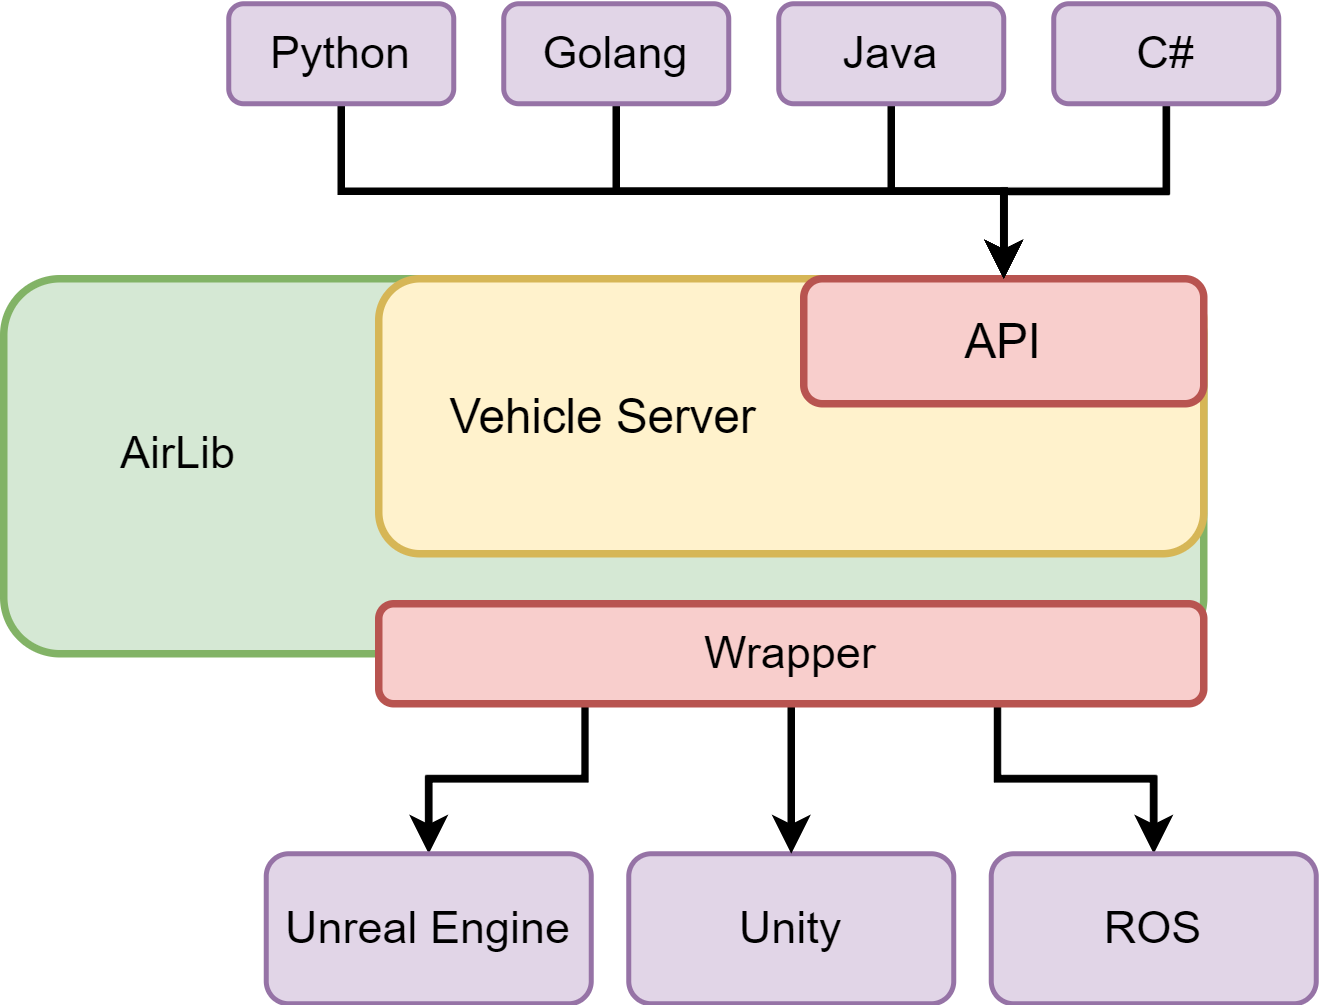
\includegraphics[width=0.5\textwidth]{05_AnalysisAndDesign/Diagrams/OriginalOverview.png}
    \caption{High-level overview of the core components of AirSim used for this project. Only one server exists.}
    \label{ADA:Figure:OriginalOverview}
\end{figure}


\subsection{AirLib}

\subsection{AirLib Wrapper}

\subsection{AirSim with Unity}

\subsection{User Interaction Layer}
AirSim allows for a variety of different languages to interact with AirLib. This is because the API calls use MessagePack\footnote{\url{https://msgpack.org/}} also known as MsgPack. MsgPack allows for an efficient binary serialisation\footnote{\url{https://github.com/msgpack/msgpack/blob/master/spec.md}}. MessagePack supports over 50 programming languages and environments. These include C\#, Golang, Haskell and others.  For this project, only Python will be used. This is because Python is a flexible language that makes prototyping quick and easy. The existing code for the user interaction layer is already written in Python, so it will be more beneficial to continue with this rather than starting from scratch.

In the Python project, three classes are implementing the APIs for each of the servers. This is to make it clear which type of entity the user is communicating with. It also avoids confusion when passing controls to the simulator, as pedestrian and vehicles use different controls. Python allows for external tools like OpenCV to process the images passed from the Simulator. Figure~\ref{} shows a diffusion map generated by OpenCV using two images created by forward-facing cameras on a car. The diffusion map highlights objects that are shifted more between the two images, i.e. the object has to be closer. 



\begin{figure}[H]
    \centering
    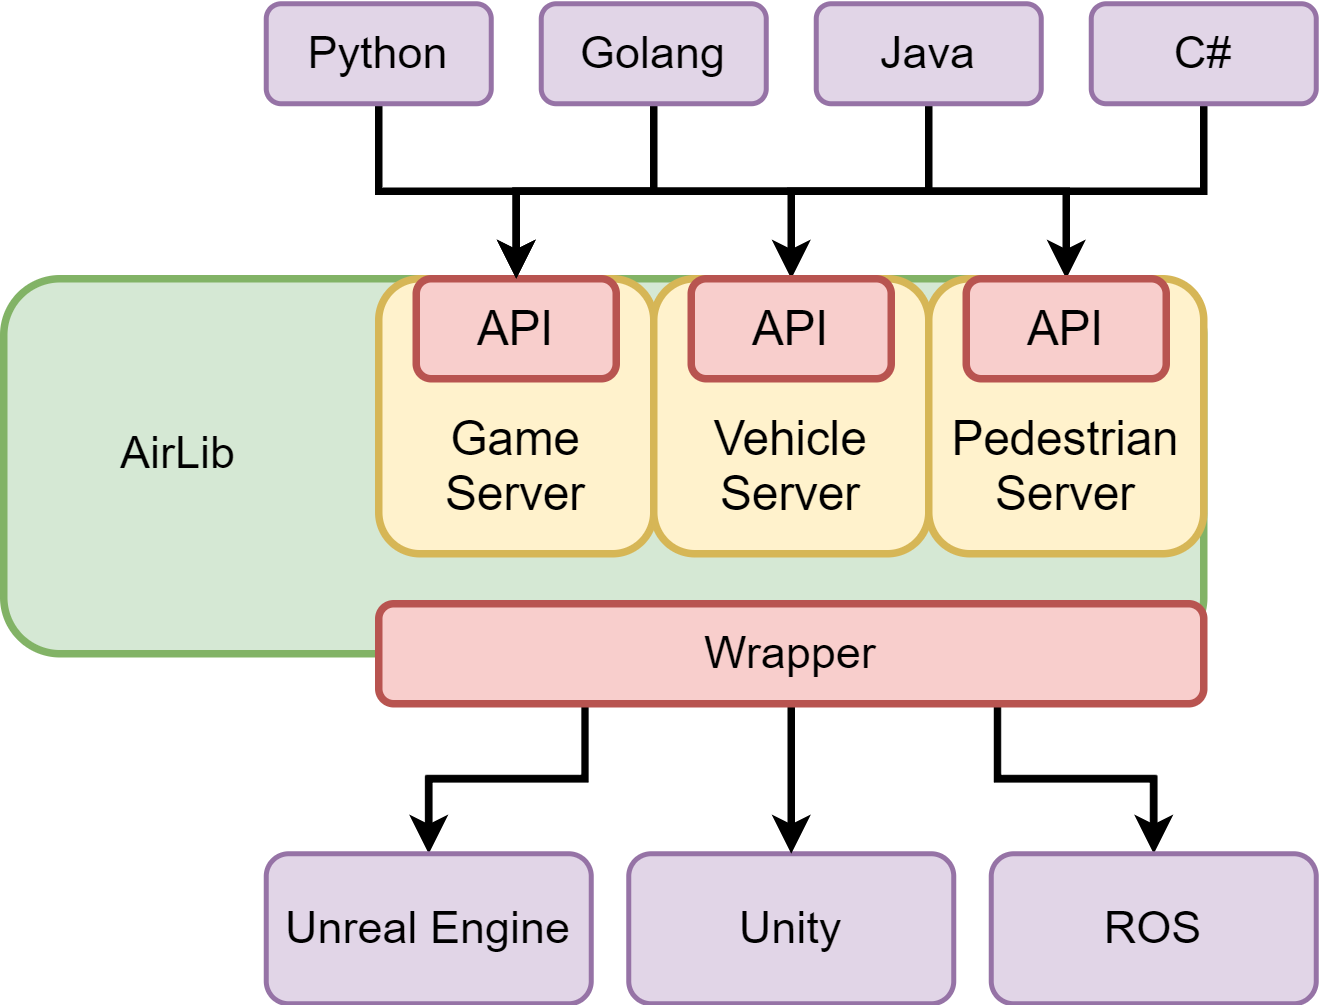
\includegraphics[width=0.7\textwidth]{05_AnalysisAndDesign/Diagrams/UpdatedOverview.png}
    \caption{Separate APIs into several servers on different ports. This makes it easier to expand the APIs and add additional features.}
\end{figure}

\begin{figure}[H]
    \centering
    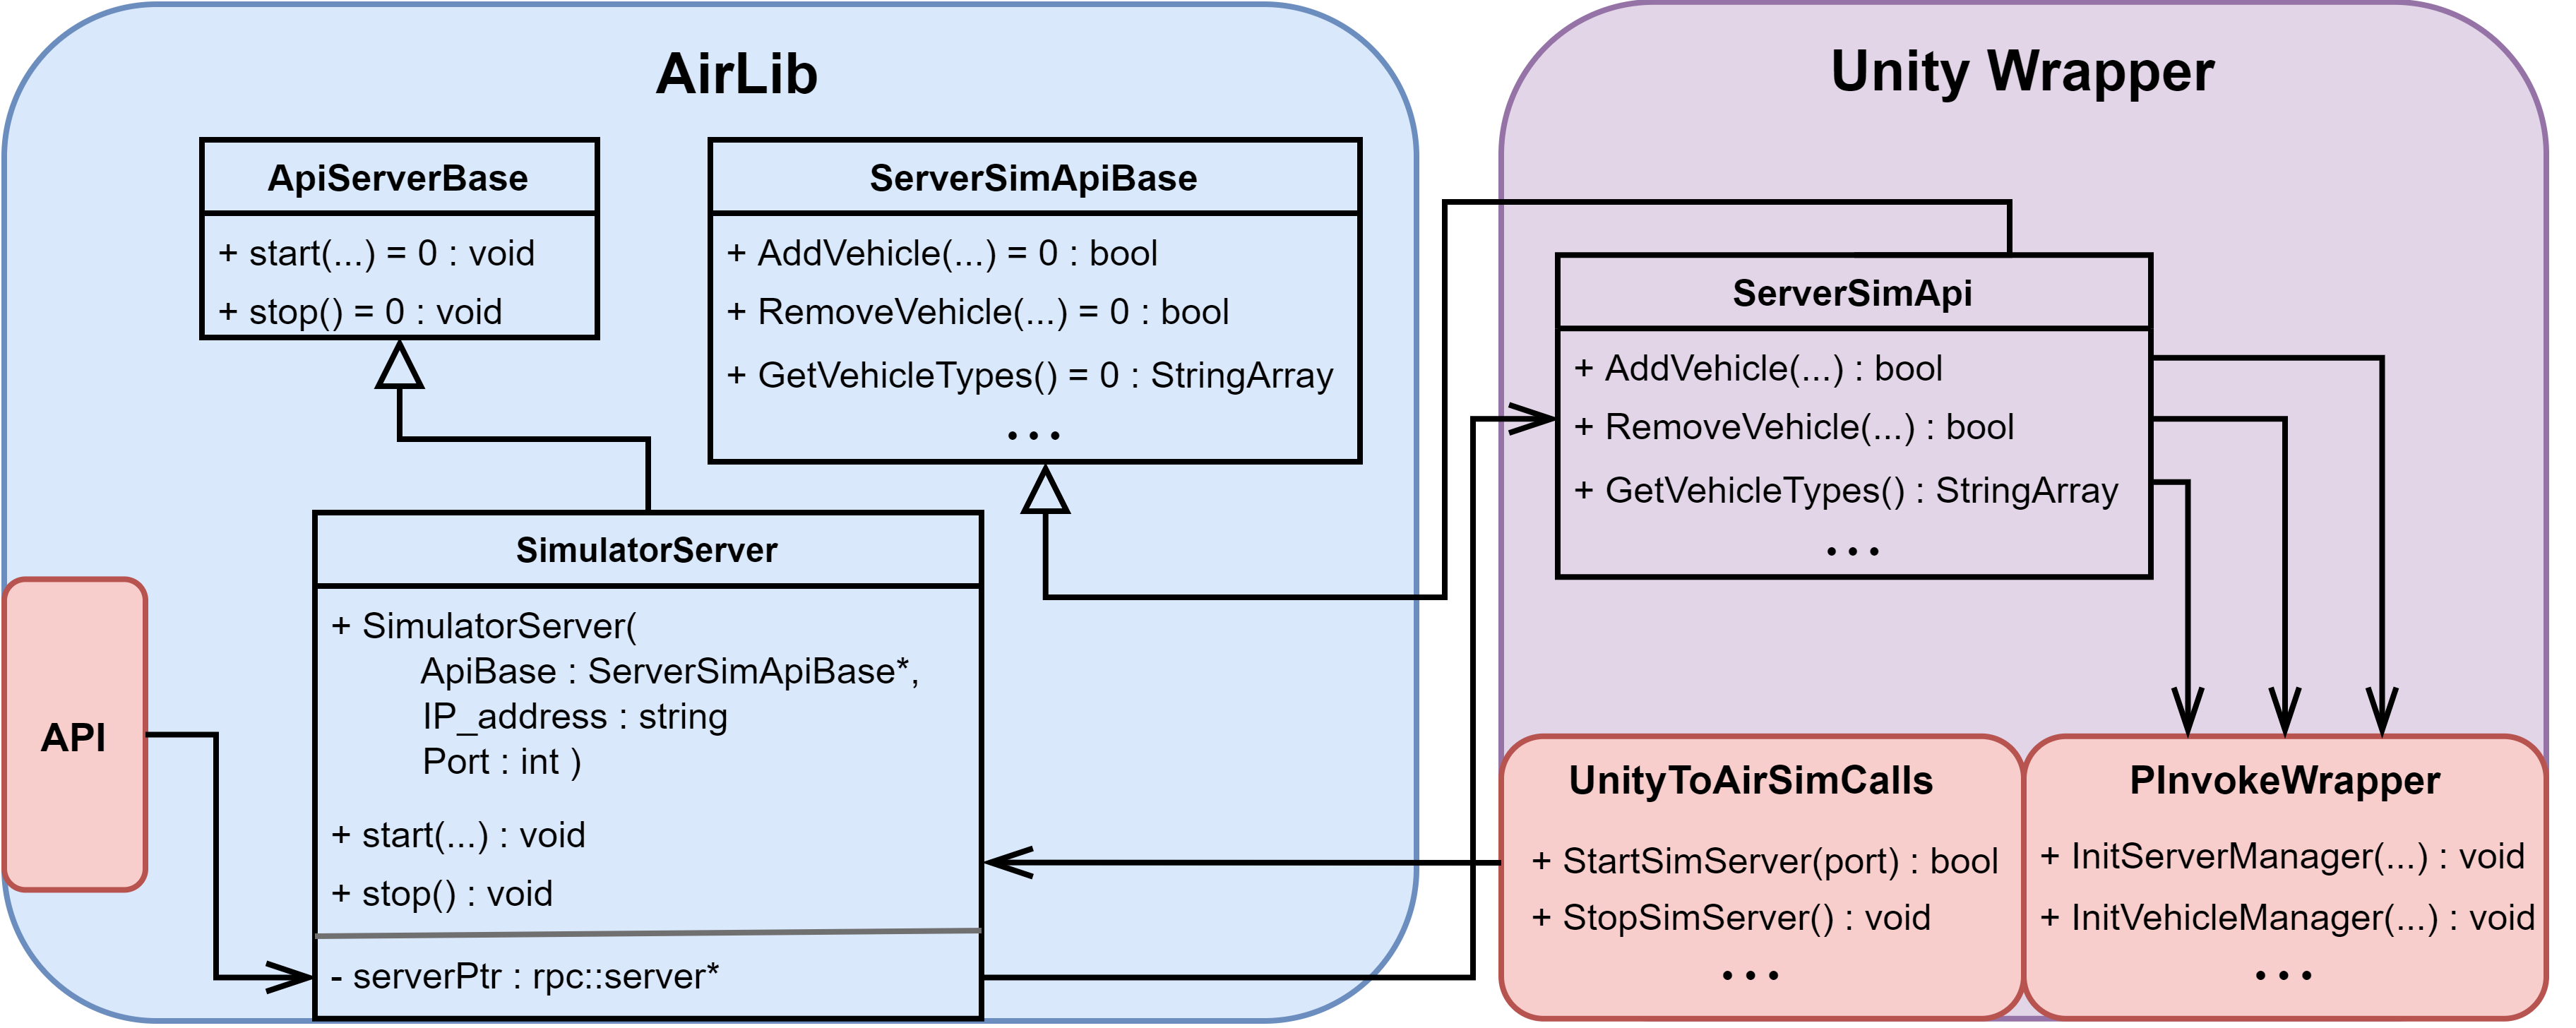
\includegraphics[width=1\textwidth]{05_AnalysisAndDesign/Diagrams/UnityWrapper2.png}
    \caption{A simplified view of how AirLib and the Unity Wrapper link together.}
\end{figure}

\begin{figure}[H]
    \centering
    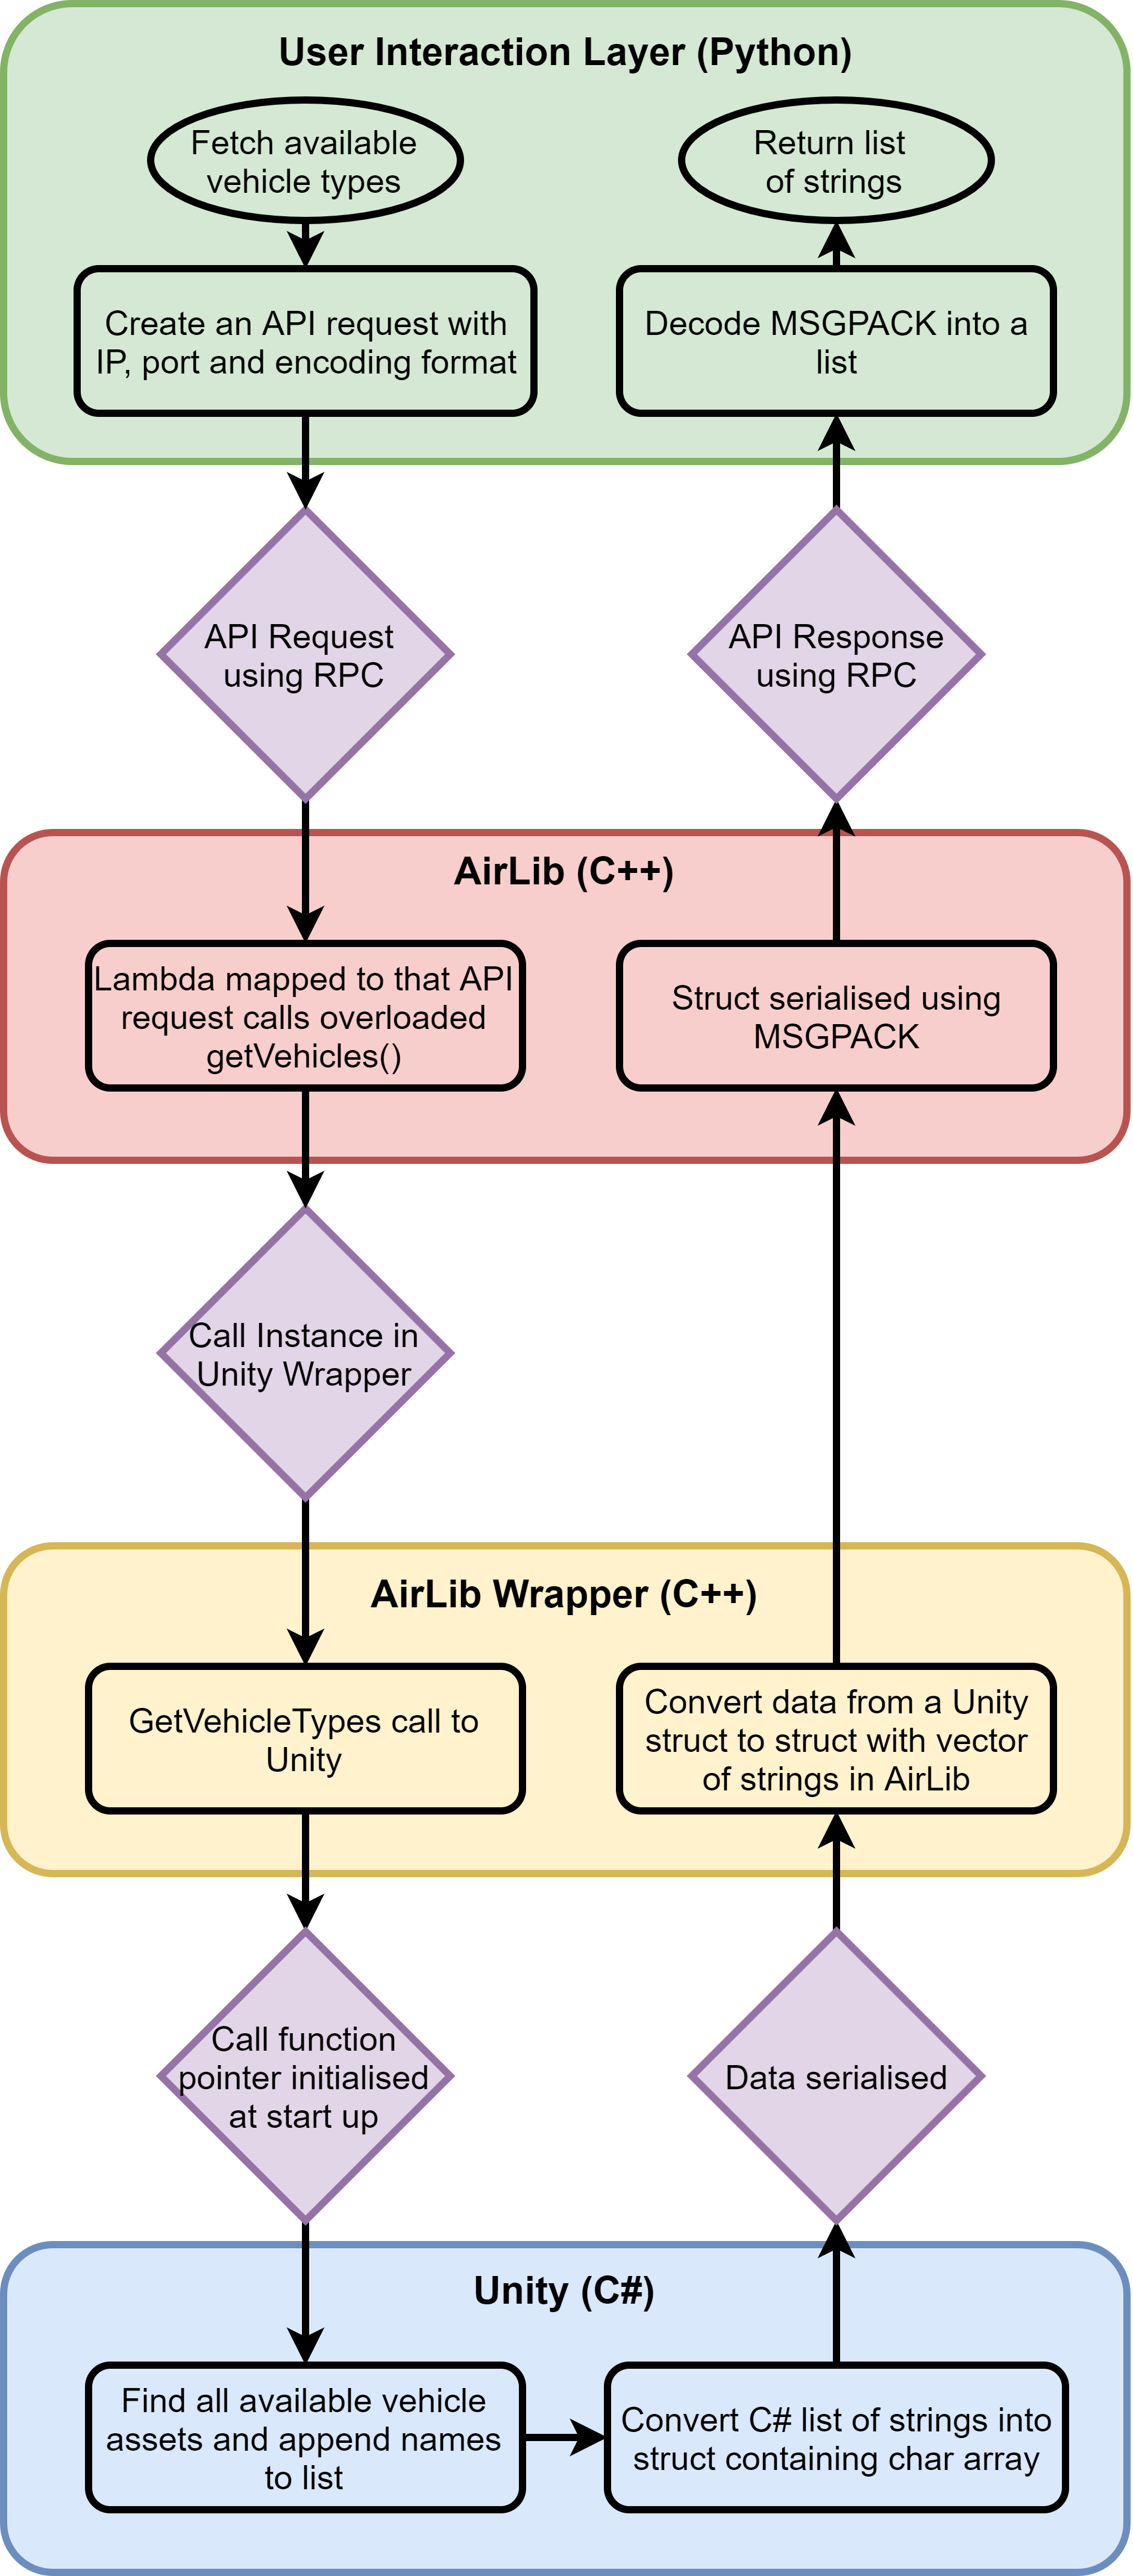
\includegraphics[width=0.6\textwidth]{05_AnalysisAndDesign/Diagrams/stringArray.png}
    \caption{High-level overview of the API that fetches available vehicle types. For APIs that require arguments, these will be encoded and added to the API request. The main change between different API requests is what happens in Unity.}
\end{figure}

\section{Architectural Design}
% Modularity
\paragraph{Dividing the server}
\paragraph{Moving logic to Unity}
\paragraph{Simplifications}
\section{Architectural Limitations}

